\section{Câu 11}
Thiết kế mạch Schmitt Trigger thực hiện đặc tuyến như ở hình 6a và 6b. (Mỗi hình 1
mạch, coi OPAMP là lý tưởng)
\begin{figure}[H]
	\centering
	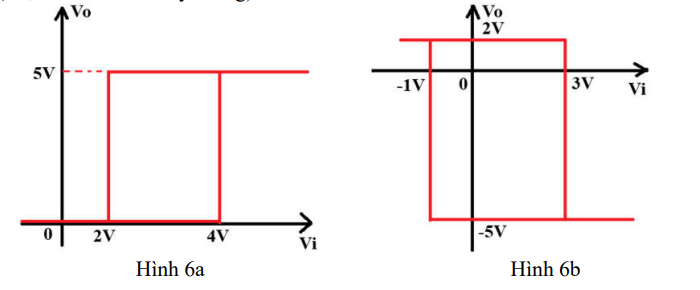
\includegraphics[scale=0.6]{image/C11_De.png}
\end{figure}

\begin{center}
\textbf{Bài giải}
\end{center}

\textbf{Hình 6a}\\
Dùng mạch Schmitt Trigger không đảo
\begin{figure}[H]
	\centering
	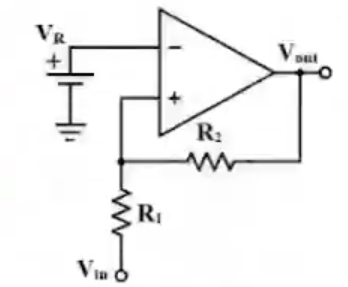
\includegraphics[scale=0.55]{image/C11_Trigger_Ko_Dao.png}
\end{figure}
Ta có:
\begin{align*}
	V_{DB} &= V_{UT} - V_{LT} = (V_{OH}-V_{OL})\dfrac{R_1}{R_2}
	&\hspace{0cm}\text{Với}\quad
	\left\{
	\begin{aligned}
		V_{UT} &= 4V\\
		V_{LT} &= 2V\\
		V_{OH} &= 5V\\
		V_{OL} &= 0V
	\end{aligned}
	\right.\\
	\rightarrow\quad   2 &= 5 \cdot \dfrac{R_1}{R_2} \quad
    \rightarrow\quad \dfrac{R_1}{R_2} = \dfrac{2}{5} 
\end{align*}

Chọn
\boxed{%
\left\{
\begin{aligned}
R_1 &= 2\ \mathrm{k}\Omega\\
R_2 &= 5\ \mathrm{k}\Omega
\end{aligned}
\right.
}\\

Có: $V_{LT} = V_R\left(1+\dfrac{R_1}{R_2}\right) - V_{OH}\dfrac{R_1}{R_2} \quad \rightarrow \quad \boxed{V_R = 2.857V}$

Mô phỏng:
\begin{figure}[H]
	\centering
	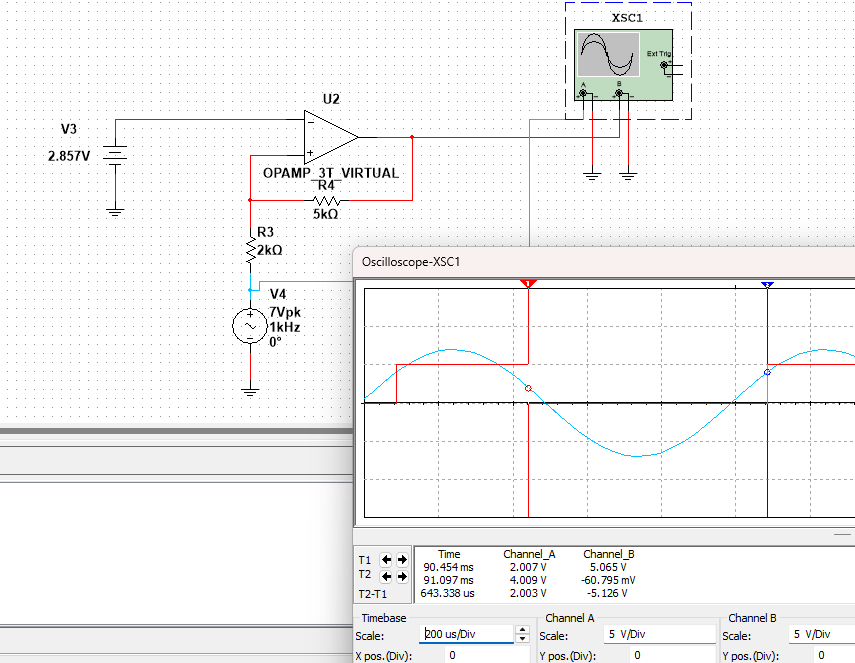
\includegraphics[scale=0.5]{image/C11_6a.png}
\end{figure}
\textbf{Nhận xét:} Với signal màu xanh là input và đỏ là ouput, có thể thấy $V_{UT}=4.009V, V_{LT}=2.007V, V_{OH}=5.065V, V_{OL}=-0.068V$ đã đúng với yêu cầu thiết kế.
Khi $V_i>V_{UT}$ thì $V_o=V_{OH}$ và khi $V_i<V_{LT}$ thì $V_o=V_{OL}$.\\

\textbf{Hình 6b}\\
Dùng mạch Schmitt Trigger đảo
\begin{figure}[H]
	\centering
	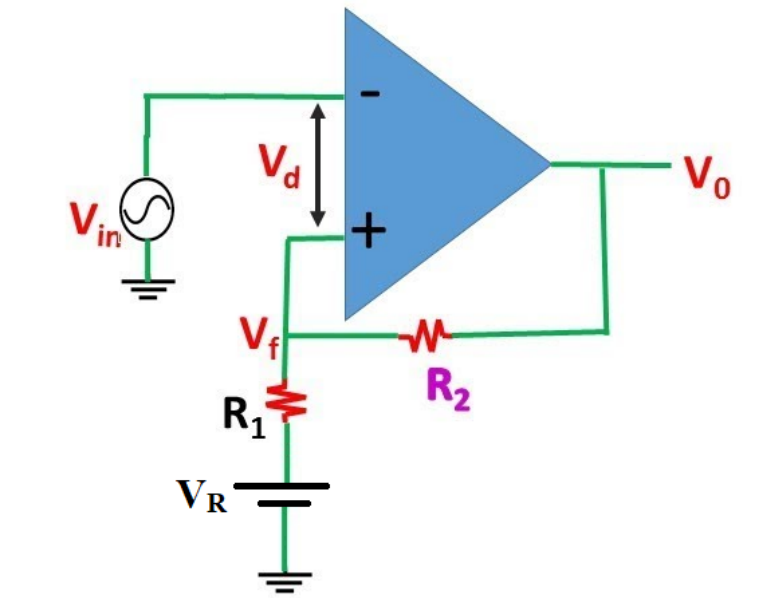
\includegraphics[scale=0.5]{image/C11_Trigger_Dao.png}
\end{figure}
Ta có:
\begin{align*}
	V_{DB} &= V_{UT} - V_{LT} = (V_{OH}-V_{OL})\dfrac{R_1}{R_1+R_2}
	&\hspace{0cm}\text{Với}\quad
	\left\{
	\begin{aligned}
		V_{UT} &= 3V\\
		V_{LT} &= -1V\\
		V_{OH} &= 2V\\
		V_{OL} &= -5V
	\end{aligned}
	\right.\\
	\rightarrow\quad   4 &= 7 \cdot \dfrac{R_1}{R_1+R_2} \quad
    \rightarrow\quad R_1 = \dfrac{4}{3}R_2  
\end{align*}

Chọn
\boxed{%
\left\{
\begin{aligned}
R_1 &= 4\ \mathrm{k}\Omega\\
R_2 &= 3\ \mathrm{k}\Omega
\end{aligned}
\right.
}\\

Có: $V_{LT} = \dfrac{V_{OL}R_1 + V_RR_2}{R_1+R_2} \quad \rightarrow \quad \boxed{V_R = 4.333V}$\\

Mô phỏng:
\begin{figure}[H]
	\centering
	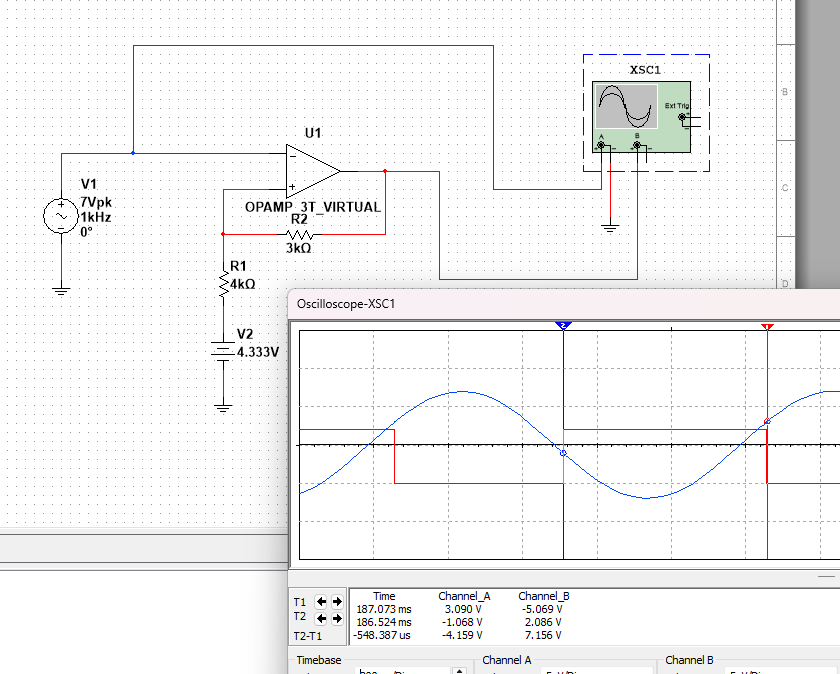
\includegraphics[scale=0.5]{image/C11_6b.png}
\end{figure}
\textbf{Nhận xét:} Với signal màu xanh là input và đỏ là ouput, có thể thấy $V_{UT}=3.090V, V_{LT}=-1.068V, V_{OH}=2.086V, V_{OL}=-5.069V$ đã đúng với yêu cầu thiết kế.
Khi $V_i>V_{UT}$ thì $V_o=V_{OL}$ và khi $V_i<V_{LT}$ thì $V_o=V_{OH}$.
